%\subsection{Einleitung}
\begin{frame}
  \frametitle{Zerlegungsmethoden}
  \framesubtitle{Teile-und-Herrsche-Strategie}
  \begin{itemize}
    \item Funktional
    \item Ressourcenorientiert
  \end{itemize}
\end{frame}

\begin{frame}
  \frametitle{Zerlegungsmethoden}
  \framesubtitle{Funktional}
  \begin{itemize}
    \item Kleinere, im besten Fall atomare, Funktionen/Prozeduren
    \item Funktionen sind von einander unabhängig
    \item Sprachen theoretisch austauschbar (Sprachen Turing-vollständig)
    \item Kosten: Zeit und Speicher
  \end{itemize} 
\end{frame}

\begin{frame}
  %\frametitle{Zerlegungsmethoden}
  \framesubtitle{Funktional}
  \begin{itemize}
    \item Funktionssignatur
    \begin{itemize}
      \item Name
      \item Parameter
      \item Rückgabetyp
      \item Bedingungen/Einschränkungen
     \end{itemize} 
    \item Funktionssemantik/-Definition
    \begin{itemize}
      \item Ausführungslogik
      \item Fehlerbehandlung
      \item Beschreibung durch Kommentare, Dokumentation oder Code
    \end{itemize} 
  \end{itemize} 
\end{frame}

\begin{frame}[fragile]
  %\frametitle{Zerlegungsmethoden}
  %\noindent\begin{minipage}{\textwidth}
  \framesubtitle{Funktional - Beispiel}
  \begin{lstlisting}[caption={Funktionssignatur},captionpos=b,label={lst:signatur}]
    function sum(a: int, b: int) -> int;
  \end{lstlisting}

  \begin{lstlisting}[caption={Funktionssemantik},captionpos=b,label={lst:semantik}]
    function sum(a: int, b: int) -> int {
        return a + b;
    }
  \end{lstlisting}
  %\end{minipage}
\end{frame}

\begin{frame}
  %\frametitle{Zerlegungsmethoden}
  \framesubtitle{Ressourcenorientiert}
  \begin{itemize}
    \item Kleinere, auf Ressourcen orientierte Sicht 
    \item Einheit auf eine bestimmte Ressource spezialisiert
    \item Nur Set von Funktionen: Basis CRUD
    \item Häufig intuitiver als Funktionen
  \end{itemize} 
\end{frame}


\begin{frame}
  %\frametitle{Zerlegungsmethoden}
  \framesubtitle{Beispiel Stuhl}
  \begin{figure}[ht]
  \centering
  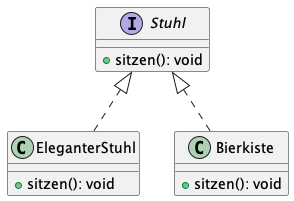
\includegraphics[width=0.3\textwidth]{fig/uml/stuhl-function.png}
  \caption{Funktionale Zerlegung mit Interface}
  \label{fig:stuhl-f}
  \end{figure}
  \begin{figure}[ht]
  \centering
  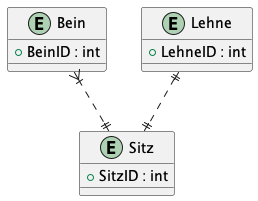
\includegraphics[width=0.3\textwidth]{fig/uml/stuhl-resourcen.png}
  \caption{Ressourcen-orientierte Zerlegung mit Relation}
  \label{fig:stuhl-r}
  \end{figure}
\end{frame}

\begin{frame}[fragile]
  %\frametitle{Zerlegungsmethoden}
  \noindent\begin{minipage}{\textwidth}
  \framesubtitle{Beispiel Schach in Code}
    \begin{lstlisting}[caption={Schachbrett - Objektorientiert},captionpos=b,label={lst:schachbrett-oo}]
    public class ChessBoard {
        private Piece[][] board;

        public ChessBoard() {
            this.board = new Piece[8][8];
            // Initialize the board with the starting positions of pieces
            // e.g. add new Piece(PieceType.ROOK, Color.WHITE) to board[0][0] for the white rook in the top-left corner.
        }

        public void setPiece(int row, int col, Piece piece) {
            board[row][col] = piece;
        }
    }
  \end{lstlisting}
  \end{minipage}
\end{frame}

\begin{frame}[fragile]
  \begin{lstlisting}[caption={Schachbrett - Datenbank},captionpos=b,label={lst:schachbrett-datenbank}]

  CREATE TABLE ChessBoard (
      id INT PRIMARY KEY,
      row INT,
      col INT,
      pieceType VARCHAR(10),
      pieceColor VARCHAR(5)
  );
\end{lstlisting}
\end{frame}
